\section{问题三的模型建立与求解}
本文针对问题三设计了一个兼顾员工技能水平提升和优化最小超时总和的\textbf{双目标优化模型},并采用\textbf{贪心算法}求解。
模型的整体框架图如\cref{fig:stru}:

\begin{figure}[h]
    \centering
    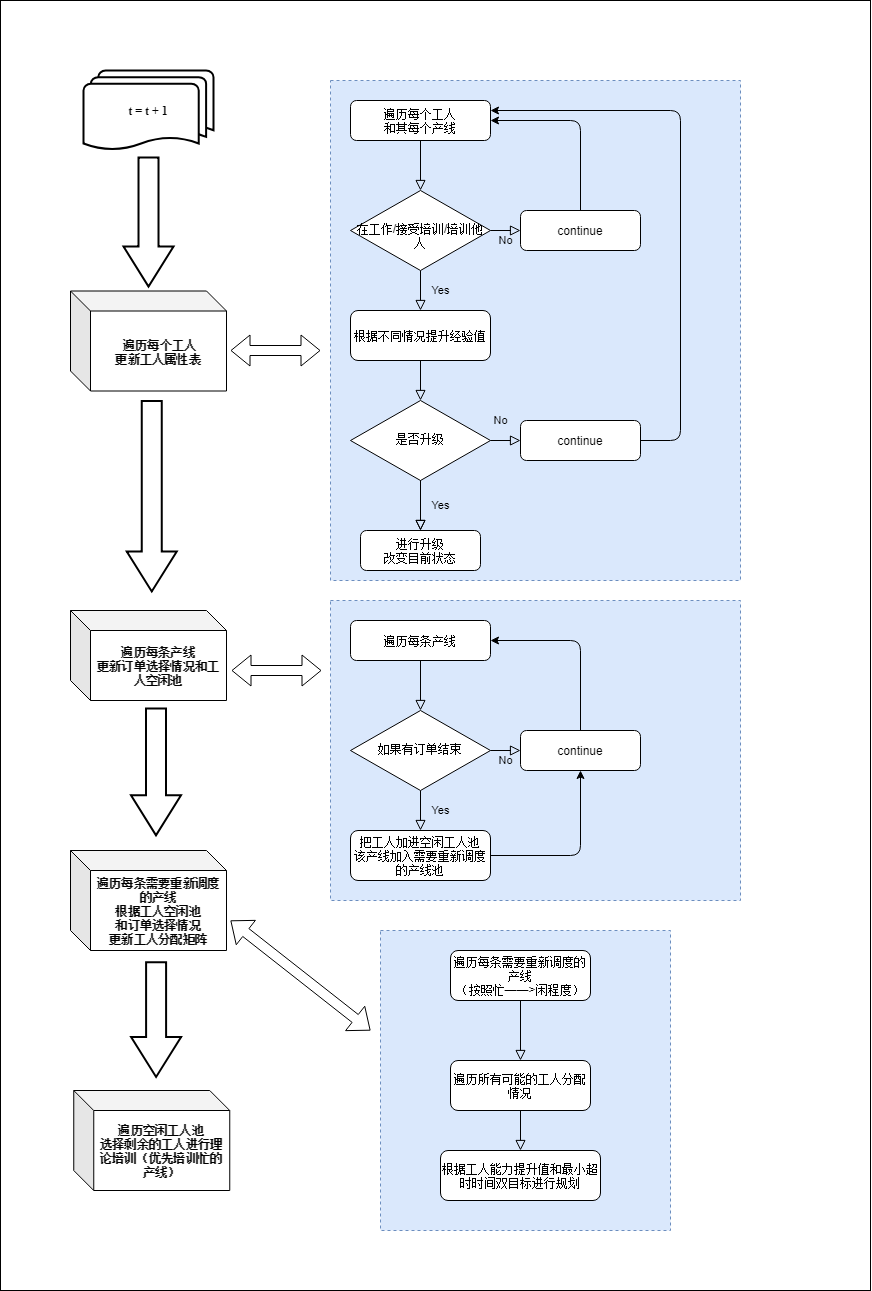
\includegraphics[height = 0.65\textheight]{pics/p4.png}
    \caption{问题三算法结构图}
    \label{fig:stru}
\end{figure}
\newpage

\subsection{员工技能水平更新}
员工技能水平更新发生在每个时间片(min),其根据时间轴的前进更新员工的技能属性指标。我们先介绍员工属性表,然后介绍技能属性的更新策略。

\subsubsection{员工属性设定}
对于每个员工,为其设置以下几个属性:

\begin{table}[htbp]
    \caption{员工属性表}
    \label{tab:worker} 
    \centering
    \begin{tabular}{@{\hspace{20pt}}c@{\hspace{40pt}}c@{\hspace{20pt}}}
        \toprule[1.5pt]
        员工属性 & 内容 \\
        \midrule[1pt]
        对产线i技能水平等级  &  N/O/E    \\
        对产线i是否完成理论培训 & 0/1          \\
        对产线i是否完成产线培训   & 0/1         \\
        目前的经验值 & exp \\
        
        \bottomrule[1.5pt]
    \end{tabular}
\end{table}

\subsubsection{更新策略}
对于员工技能水平更新,考虑以下几点:
\begin{enumerate}[left=2em]
    \item 对于当前正在工作的员工,更新其技能水平。
    \item 对当前未工作的员工,更新其理论提升水平。
    \item 如果该员工某条产线的技能水平达到了一个阈值,则提升该员工的技能等级。
\end{enumerate}

\subsection{产线分配订单更新}
产线分配订单更新的流程如下:

在每一个时间片(1min),分别考虑每一条产线,检查是否有订单被完成。如果有订单被完成:

\begin{enumerate}[left=2em]
    \item 把其对应的员工放到员工空闲池中,修改对应员工的工作状态,并且把该产线标记为需要重新分配员工。
    \item 根据第一问的调度算法确定下一个应该选择的订单。
\end{enumerate}


\subsection{产线分配员工更新}

在确定了哪些产线需要重新分配员工之后,采用第二问的算法,根据产线的繁忙情况确定优先分配员工的产线顺序,随后根据空闲员工池情况确定所有可以分配的空员工组合,然后通过遍历所有组合求解员工提升水平和最小超时时间和的双目标优化问题,得到当前产线的分配员工情况。

\subsubsection{所有可分配的员工组合的确认}

对于空闲员工池中所有的空闲员工,首先遍历出所有的组合,对每一种组合,定义满足如下条件的为可分配组合:

\begin{itemize}[left=1em]
    \item 如果有员工等级为N,其需要已经完成了理论培训,且再在空闲员工池中找一个O/E级员工对其进行培训。
    \item 对上述情况,每一个可以O/E级员工作为培训老师都是一种组合。
\end{itemize}



\subsubsection{结合员工提升水平和订单超时总和的双目标贪心员工分配模型}

对具体到每个订单的所有可分配空闲员工组合$Group_i$,定义该组合的\textbf{分配价值($Value_i$)}为:

\[
    \begin{cases}
      Value_i = impro_i  - badtime_i \\
       badtime_i = besttime - realtime_i \\
       impro_i = \sum_{k \in Workers_i} (pracimpro_k  - theomiss_k  + upgrade_k  )\\ 
       upgrade_k = upgrade_scoreO / upgrade_scoreE \quad if \quad upgrade \quad happens \\
       practimpro_k =  realtime * ratiop_{Level_{k-j}}\\
       theomiss_k = \frac{1}{12} \sum_{j=1}^{12} realtime * ratiot\quad \text{if} \quad Level_{k-j} == N 
    \end{cases}
\]

其中分配价值主要由\textbf{技能提升正价值($impro_i$)}和\textbf{超时负价值($badtime_i$)}构成。

\textbf{技能提升正价值}由员工的\textbf{实践提升水平($pracimpro_k$)}和\textbf{理论提升水平($theomiss_k$}, 由于此时分配的是生产的员工,设置为错过时间)和\textbf{升级利益($upgrade_k$)}构成,其中实践提升水平和理论提升水平与工作时间成正比,并具有不同的系数。升级利益是一个直接增加的值。

本模型的系数设置为:

\begin{table}[htbp]
    \caption{系数设置表}
    \label{tab:ratio} 
    \centering
    \begin{tabular}{c|ccccc}
        \toprule[1.5pt]
        系数 & 理论系数 & 实践系数OE& 实践系数NO&
        升级利益OE&
        升级利益NO\\
        \midrule[1pt]
        设置值  & 0.1 &  0.2 & 0.3 & 1000 & 500     \\
        \bottomrule[1.5pt]
    \end{tabular}
\end{table}


\textbf{超时负价值}由该员工组合的\textbf{实际工作时间}和该订单的\textbf{最少工作时间}(即所有员工全部为E且不参与培训)的差值计算得到。

考虑到两者的量纲相同,我们将其设置为两种价值直接相减得到。在每一次分配员工的时候,都会遍历目前所有的组合,并选取\textbf{分配价值}最高的员工组合进行分配。

\subsection{空闲员工池处理}

在分配完目前的所有订单后,对于空闲员工池中还剩余的员工,我们对其进行理论培训。按照产线的繁忙程度优先培训繁忙产线的空闲N级员工。

\subsection{模型总结}

本问题采用的模型以员工技能水平的提升为主要考虑点,将订单超时时间总和作为次要优化点(在双目标函数中为员工的技能提升设置了较大的系数),利用、\textbf{多层次贪心}的思想求最优分配方法,其中主要包括:

\begin{itemize}[left=1em]
    \item \textbf{对产线的贪心。}在将员工分配给产线时及在选择员工培训的时候,优先考虑分配更加繁忙的产线。
    \item \textbf{对订单的贪心。}在选择下一个处理的订单时,优先考虑会使超时订单总数最小,需要的工作时间最少的订单。
    \item \textbf{对员工技能水平的贪心。}通过设置不同的系数在选择培训时优先将员工的技能水平从N提升到O
\end{itemize}

\subsection{模型求解结果}
模型最终得到的超时分钟数之和为 4033504.833。分配方案部分见\cref{tab:problem3},完整见附件。



